\documentclass[12pt]{article}
\usepackage[spanish]{babel}
\usepackage[utf8]{inputenc}
\usepackage[T1]{fontenc}
\usepackage{graphicx,amsmath,amsfonts,amssymb,epsfig,euscript}
\usepackage{cite}
\usepackage{float}
\usepackage{geometry}
\usepackage{subfig}
\usepackage{parskip}
\usepackage{tikz}
\usepackage{pgfplots}
\usepackage{color}
\usepackage{listings}
\usetikzlibrary{calc}
\graphicspath{{IMAGES}}
\newcommand{\myref}[1]{\color{blue}\bf(\ref{#1})}
\newtheorem{tab}{Tabla}
\renewcommand\tablename{Tabla}
\setlength{\columnsep}{7mm}
\renewcommand\tablename{Tabla}
\renewcommand\contentsname{\'Indice}
\setlength{\topmargin}{-0.75in} \setlength{\textheight}{9.25in}
\setlength{\oddsidemargin}{0.0in} \setlength{\evensidemargin}{0.0in}
\setlength{\textwidth}{6.5in}
%%%%%%%%%%%%%%%%%%%%%%%%%%%%%%%%%%%%%%%%%%%%%%%%%%%%%%%%%%%%%

%%%%%%%%%%%%%%%%%%%%%
\usepackage{enumitem}
\renewcommand{\theenumi}{\alph{enumi}}
\renewcommand\labelenumi{\theenumi)}

\newtheorem{ejer}{Ejercicio}
\newcommand{\bej}{\begin{ejer}\rm}
	\newcommand{\fej}{\end{ejer}}


\newcommand{\R}{\mathbb{R}}
\newcommand{\C}{\mathbb{C}}
\def\dt{\Delta t}
\def\dx{\Delta x}

\topmargin-2cm \vsize 29.5cm \hsize 21cm
\setlength{\textwidth}{17.00cm}\setlength{\textheight}{23.5cm}
\setlength{\oddsidemargin}{0.0cm}
\setlength{\evensidemargin}{0.0cm}
%%%%%%%%%%%%%%%%%%%%%%%%%%%%%%%%%%%%%

\begin{document}

\title{Implementación del método de elementos finítos para la solución numérica de la ecuación de Black-Scholes.}
\author{Lester Armando Vallecillo M.}

\date{30 de Abril del 2020}

\twocolumn[
\begin{@twocolumnfalse}
\maketitle
\vspace*{-0.8cm}
\begin{center}\rule{0.9\textwidth}{0.1mm} \end{center}
\begin{abstract}
\normalsize

En la actualidad, una variabilidad de problemas en diferentes campos de estudio requiere la necesidad de buscar mecanismos que permitan obtener mejores resultados para la toma de decisiones. Ciertamente, la modelización de algunos problemas es dinámica y está consolidada en fundamentos matemáticos. Espesificamente, estos problemas se pueden modelar sobre estructuras de dominio espacial, y además, temporal. Usualmente, las ecuaciones diferenciales rigen el comportamiento de un gran numero de fenómenos físicos. Normalmente, no es factible encontrar la solución exacta de estos problemas y como alternativa existen métodos numericos que permiten obtener la resolución numerica, y por tanto, realizar una simulación de su comportamiento. Una herramienta precisa en el calculo y útil para optimizar el costo computacional y tiempo de ejecución en este tipo de problema, es el método numérico de los elementos finitos.\\ 

Particularmente, en los derivados financieros se destaca la ecuación de Black-Scholes, el cual modela variaciones de precios, y se basa ampliamente en la teoría de procesos estocásticos con dominio espacial, y temporal. Este modelo se representa mediante ecuaciones diferenciales de segundo orden, el cual se pueden asociar a un problema de valor inicial y de frontera. Por ejemplo, un caso particular es el problema transitorio que representa la ecuación siguiente: 
\begin{equation*} 
\left\{
\begin{array}{c}
%%%%%%%%%%%%%%
\frac{\partial{V}}{\partial{t}} + \frac{{\sigma}^2}{2}\frac{\partial^2{V}}{\partial{x^2}}
+ r\frac{\partial{V}}{\partial{x}}-rV=0,\\ \\
\phi(x_t) = \max{(K-x_t,0)} 
\end{array} \right.
%%%%%%%%%%%%%%%%%  
\end{equation*}
Donde $ \frac{{\sigma}^2}{2}\frac{\partial^2{V}}{\partial{x^2}}$, $r\frac{\partial V}{\partial x}$ y $-rV$ son las componentes de difusión, convección y reacción.\\

En el presente artículo se pretende describir algunos fundamentos del modelo Black-Scholes y del método de los elementos finitos para obtener la resolución del problema transitorio implícito en el modelo de ganancia \textit{put}, justificando el uso de sus tecnicas y aplicaciones en el marco teórico. De la misma manera, se pretende ilustrar el uso de un algoritmo para su implementación computacional y de esta manera, simular el comportamiento del fenómeno que describe dicha ecuación. 

     
\begin{center} \rule{0.9\textwidth}{0.1mm} \end{center}
\vspace*{0.3cm}
\end{abstract}

\end{@twocolumnfalse}]


%%%%%%%%%%%%%% SECCION INTRODUCCION %%%%%%%%%%%%%%%%%%%%%%%%%%%5
\section*{Introducci\'on}
La aplicación del método de los elementos finitos (MEF) en los diferentes campos de estudio para resolver problemas de ecuaciones diferenciales, permiten describir el comportamiento de un gran numero de fenómenos estudiados. Lo anterior,  es causa de inspiración para enunciar, deducir y desarrollar algunos resultados en los cuales se basa la teoría y sus técnicas de aproximación. El objeto de estudio es implementar esta herramienta para aproximar la solución del problema transitorio de Black-Scholes con ganancia \textit{put} y su procedimiento se describe en a continuación:
\begin{figure}[h] 
	\centering	
	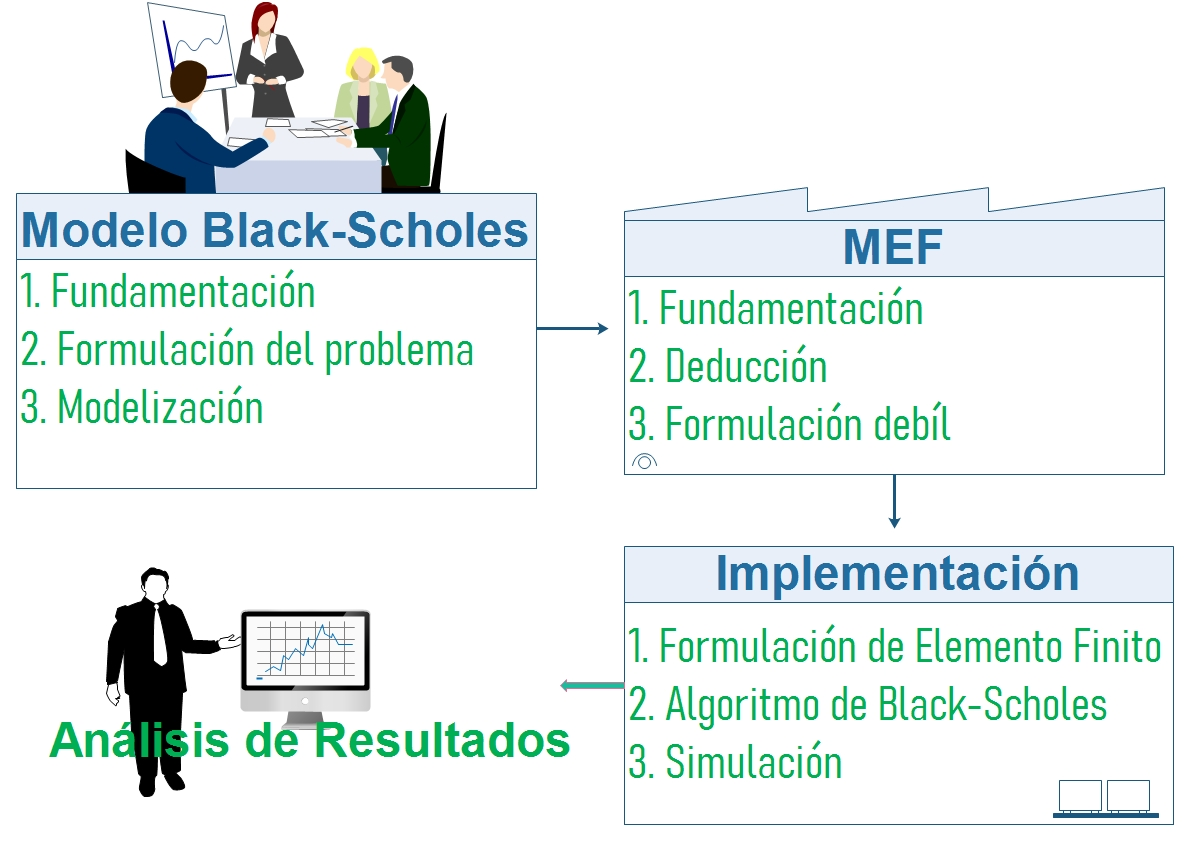
\includegraphics[width=8cm,height=6cm]{Pic/Diagr01} 
	\label{Diagrama01}.
	\caption{Metodología de implementación de MEF a el Modelo Black-Scholes. [F: Propia]}
	\hrule
\end{figure}
 
 En la primera sección \ref{Sec:01}, se exponen algunos conceptos de problemas de valoración de opciones, específicamente del modelo de Black-Scholes de opción europea (\textit{call}), y se deduce la ecuación diferencial equivalente, deduciendo algunos resultados fundamentales, para luego, encontrar la ecuación del calor asociada a este problema.\\
 
 En la sección \ref{Sec:02}, se describen algunos aspectos teóricos y prácticos relacionados con el método numérico de los elementos finitos, deduciendo así, algunos resultados importantes para comprender su utilidad y técnicas de aproximación. En conseccuencia, Se desarrolla la formulación débil del problema clásico. Luego, se ilustra la idea de formulación del problema de elemento finito. Finalmente, se deduce un algoritmo de implementación que permite obtener la resolución del problema. 
 
%%%%%%%%%%%%%%%%%%% ANTECEDENTES  %%%%%%%%%%%%%%%%%%%%%%%%%%%%% 
\section*{Antecedentes}
En 1900, Bachelier tuvo el primer intento de modelización matemática en los mercados financieros con el desarrollo de una teoría de valoración de opciones \cite{Art03}. Defendió su tesis doctoral "Théorie de la Spéculation", supervisado por Henri Poincaré y en la cual  utilizó argumentos de probabilidad para introducir que los precios de los activos siguen un movimiento browniano con deriva \cite{Lib02}. Ciertamente, su tesis no fue valorada, sino hasta 1973 cuando se publica el artículo de Robert Merton \cite{Lib06}, en el cual hacía referencia a los trabajos de Fischer Black y Myron Scholes \cite{Lib05} y que incluye una fórmula analítica para valorar un tipo específico de opciones.\\

Por otra parte, en 1915, B. Galerkin propuso el método numérico MEF y fue denominado como el método de Galerkin. En 1943, R. Courant propone utilizar funciones polinómicas en subregiones triangulares, como método especial del problema variacional de Rayleigh-Ritz para aproximar soluciones. En la década de los 60, el método  se hace popular, gracias a su efectiva aplicación en los diferentes campos de estudio, principalmente de ingeniera, con un importante avance en el calculo de la resolución de algunos problemas, gracias a su mejoramiento en la precisión, optimización de tiempo y memoria de ordenadores. Su evolución,  se describe en una linea de tiempo, ver en Anexos la Figura \ref{Fig:01}. 
  
%%%%%%%%%%%%%%%%% MODELO BACK-SCHOLES %%%%%%%%%%%%%%%%%%%%%%%%
\section{El Modelo Back-Scholes}\label{Sec:01}
Se introduce los fundamentos teóricos relacionados con el problema de valoración de opciones o derivados financieros. De la misma manera, se presenta la ecuación de Back-Scholes como un problema transitorio de valor inicial y de frontera.\\

%%%%%%%%%%%%% Valoración de Opciones %%%%%%%%%%%%%%%%%%%%%%%%%%
\subsection{Valoración de Opciones}
Los usuarios y entidades financieros deben evaluar el riesgo ante la toma de decisiones estratégicas \cite{Art01}. Por tanto, gestionar contratos que generen ganancias a través del tiempo requiere de una variabilidad de condiciones. 

Algunos acuerdos se denominan opciones, y son instrumentos financieros derivados que otorgan al propietario o comprador(holder) el derecho y al vendedor(writer) la obligación de realizar la transacción a un precio fijado en un periodo de tiempo determinado, además el comprador debe pagar el derecho al vendedor por la obligación que éste adquiere cuando subscriben el contrato. Ahora bien, el holder se ve en la necesidad de estimar la cantidad a pagar, es decir, debé valorar la opción \cite{Art01}. 
%%%%%%%%%%%%% Conceptos Previos %%%%%%%%%%%%%%%%%%%%%%%%%%%%%%%
\subsection{Conceptos y Delimitaciones}\label{Sec:limitaciones}
Los activos son recursos controlados por la entidad,  la ganacia call es opción sobre una posible compra, put es opción sobre una posible venta, strike(k) el precio de ejercicio ó ejecución, subyacente(S) es el valor del subyacente, expiry date(T) la fecha expira el contrato y payoff(V) es la ganancia de los derivados.   
 
\paragraph{Delimitaciones}
Antes de introducir la ecuación, se consideran algunas hipótesis como tasa de interés(r) y volatilidad($\sigma$) son constantes, no hay costes de transacción, la acción no paga dividendos, se permiten ventas en corto, no hay oportunidad de arbitraje y la distribución de retornos es normal.
%%%%%%%%%%% El Modelo Back-Scholes %%%%%%%%%%%%%%%%%%%%%%%%%%%%
\subsection{La ecuación Back-Scholes}
Se pretende encontrar una formulación que ajuste el precio de los distintos tipos de acuerdos, durante un periodo de tiempo. Inicialmente, se considera para el modelo de valoración de opciones europea con ganancia \textit{call} las condiciones siguientes:
\begin{description}
	\item[ $S_t < K$] El holder ejerce la opción para adquirir el subyacente y la ganancia $\phi(S_t)$ seria $S_t-K$. 
	\item[ $S_t \geq K$] El holder no ejerce la opción porque no obtiene ganancia, es decir, $\phi(S_t)$ es nula.
\end{description}  
Lo anterior, se puede expresar como:
\[  \phi(S_t) = \max{(S_t-K,0)}  \]
Donde, $S_t$ es el valor del activo en la fecha de expiración $\textit{t}$ y $\phi(S_t)$ es la ganancia. De manera similar, en el caso de opción \textit{put}, se deduce la ganancia como: 
\[ 
\phi(S_t) = \max{(K-S_t,0)}
\]

% El precio subyacente del activo.
Se puede modelar el precio del activo mediante procesos estocásticos en un periodo. En consecuencia, esto nos permite establecer un espacio de probabilidades $(\Omega, F,\textit{p})$, donde $\Omega$ es el conjunto de eventos, $F$ es una $\sigma-Algebra$ que contiene todos los eventos posibles y \textit{p} es función que asigna una probabilidad a cada $\textit{f} \in F$. Lo anterior, se conoce como proceso de Markov. De donde, una propiedad establece que $E[x_s|F_t] = E[x_s|x_t]$, para toda función medible acotada, $s \geq t$ y $x_t \in X$, donde $X = \{ x_t : t \in [0,\textit{T}] \}$, el proceso implica un comportamiento de $X$, es decir, que el valor del activo subyacente en el tiempo \textit{t} depende del $x_t$ anterior y mediante procesos de Wiener se puede modelar la evolución del precio por ecuaciones diferenciales estocásticas con parte determinista y particularmente se puede representar como:  
\begin{equation}
ds_t = \alpha(x,t) s_t dt + \beta(x,t) s_t dw(t) 
\label{Ecu:01}
\end{equation}
Donde $W = \{w_t : t\geq 0\}$ es un proceso de Wiener, $\alpha(x,t)$ es la tendencia y $\beta(x,t)$ la volatilidad. De la misma manera, si se define la tasa de retorno como $ds/s$, esta ecuación describe el movimiento Browniano, donde la componente determinista $ds/dt=\alpha(x,t)s$ tiene por solución analítica $s_t = s_0 e^{\alpha(x,t)(t-t_0)}$.

Un resultado fundamental es el Lema de Ito que establece una identidad usada para encontrar el diferencial de una función dependiente del tiempo de un proceso estocástico \cite{Lib07}. Es decir, el precio sigue un movimiento Browniano y sus cambios instantáneos están determinados por la ecuación \eqref{Ecu:01}. Entonces $y_t = g(x_t,t)$ verifica la identidad siguiente,
\begin{equation*} 
dy_t = (\dfrac{\partial{g}}{\partial{t}} + \alpha \dfrac{\partial{g}}{\partial{x}} + \frac{1}{2}\beta^2\dfrac{\partial^2{g}}{\partial{x^2}})dt + \beta \dfrac{\partial{g}}{\partial{x}} dw(t) 
\label{Ecu:02}
\end{equation*}
Estó permite construir un modelo particular en el cual se pretende encontrar una función que cuantifica el valor de las opciones y se denota por $V(s,t)$. En consecuencia del Lema de Ito y \eqref{Ecu:01} se deduce la formula del diferencial para la función  $V$ de manera siguiente, 
\begin{equation*} 
dV = (\dfrac{\partial{V}}{\partial{t}} + \alpha s \dfrac{\partial{V}}{\partial{s}} + \frac{1}{2}\beta^2s^2\dfrac{\partial^2{V}}{\partial{s^2}})dt + \beta s \dfrac{\partial{V}}{\partial{s}} dw(t) 
\label{Ecu:03}
\end{equation*}
La modelización de Black-Scholes consiste en construir una cartera de inversión en una cantidad $\Delta$ de activos. La variaron en cada incremento ($dt$) del Portfolio $d\varPi = dV-\Delta ds$. De donde, se deduce que $\Delta =\partial{V}/\partial{s}$. Entonces, si se invierte $\varPi $ en un producto, el resultado seria $\textit{r}\varPi dt$. Ahora, si se remplaza adecuadamente las expresiones $dV$, $ds$ y $\Delta$ en la ecuación, note que $\Delta$ permite eliminar la componente estocástica de variacion de $d\varPi$  \ref{Ecu:03}. Por lo tanto, se remplazan estas expresiones en $\textit{r}\varPi dt$ y como resultado se obtiene el problema estacionario de Black-Scholes con Payoff \textit{put} que se representa así:
\begin{equation} 
\left\{
\begin{array}{c}
%%%%%%%%%%%%%%
\frac{\partial{V}}{\partial{t}} + \frac{{\sigma}^2}{2}\frac{\partial^2{V}}{\partial{x^2}}
+ r\frac{\partial{V}}{\partial{x}}-rV=0,\\
\phi(x_t) = \max{(K-x_t,0)} 
\end{array} \right.
\label{Ecu:04}
%%%%%%%%%%%%%%%%%  
\end{equation}
Donde $ \frac{{\sigma}^2}{2}\frac{\partial^2{V}}{\partial{x^2}}$, $r\frac{\partial V}{\partial x}$ y $-rV$ son las componentes de difusión, convección y reacción, respectivamente.
%%%%%%%%%%%%%%%%%%%%%%%%%%%%%%%%%%%%%%%%%%%%%%%%%%%%%%%%%%%%%%%
\subsection{El Problema de Valor Inicial Asociado}
La ecuación de Black-Scholes se puede representar en formulación explicita. El procedimiento consiste en realizar los cambios de variables $\tau = t-t_k $, $x = log(s) $, $W(x,\tau) = e^{-\tau r}V(x,\tau) $, $z = x + (r-\frac{\sigma}{2})\tau$ y $U(z,\tau) = W(x,\tau) $. Posteriormente, derivar de forma adecuada, remplazar en dicha ecuación y realizar las simplificaciones precisas. De donde, se puede asociar la ecuación \eqref{Ecu:04} se obtiene la expresión siguiente:
\begin{equation*} 
-\dfrac{\partial{U}}{\partial{\tau}} - (r-\frac{\beta^2}{2})\dfrac{\partial{U}}{\partial{z}} + \frac{1}{2}\beta^2\dfrac{\partial^2{U}}{\partial{z^2}} +
(r-\frac{\beta^2}{2})\dfrac{\partial{U}}{\partial{z}} = 0
\end{equation*}
Además, se debé considerar los efectos de los cambios de variable a la función $\phi(s_t)$. De donde, se obtiene $U(z,0) = \phi(z)$. En conclusión, el problema equivalente a la ecuación de Black-Scholes \eqref{Ecu:04} es la ecuación del calor, la cual tiene solución analítica y se representa de la forma:   
\begin{equation} 
\left\{
\begin{array}{c}
%..........................................................
\dfrac{\partial{U}}{\partial{\tau}} = \frac{\beta^2}{2}\dfrac{\partial^2{U}}{\partial{z^2}}\\[0.5cm]
U(z,0) = \phi(z)
\label{Ecu:06}
\end{array} \right.  
\end{equation}
%%%%%%%%%%%%%%%% METODO DE LOS ELEMENTOS FINITOS %%%%%%%%%%%%%%
 \section{Método de Elementos Finitos}\label{Sec:02}
MEF es una herramienta útil y precisa que permite obtener una aproximación numérica en alguna estructura, sobre la cual están definidas ciertas ecuaciones diferenciales, problemas de análisis estructural e ingieneria. La base de MEF es la formulación débil en problemas lineales simetricos.
\subsection{Conceptos basicos}
El MEF tiene como base teórica algunos conceptos del análisis funcional, numérico y de álgebra lineal, principalmente de espacios de Hilbert, ver en \cite{Lib04}. 

{\bf Definición: } {\em Un \textbf{producto interior} sobre un espacio vectorial $V$ es una forma bilineal simétrica y definida positiva.}

{\bf Definición: }{\em Si $V$ es un espacio normado completo con norma inducida por un producto interior, entonces se dice que $(V,\left\|.\right\|)$ es un \textbf{espacio de Hilbert}.}

{\bf Teorema de Proyección:}{\em Sea $H$ un espacio de Hilbert y $M\subset H$ cerrado. Dado un vector $\textit{x} \in H$, existe un $m_0 \in M$ único, tal que:
\[\left\| \hat{x}- m_0\right \| \leq \left\| x-m\right\|\]
para toda $m \in M$. Además, una condición necesaria y suficiente para que $m_0 \in M$ sea el único vector minimizante es que el error $\textit{x}-m_0$ sea ortogonal a $M$. }

%%%%%%%%%%%%%%%%%%%%%%%%%%%%%%%%%%%%%%%%%5

\subsection{Aspectos Teóricos y Prácticos relacionados con MEF}
Para enunciar las técnicas de aproximación del método se asume el lector esta familiarizado con la base teórica. Habitualmente, para deducir la formulación débil se utiliza el problema \textit{clásico estacionario} siguiente:
\begin{equation} 
\left\{
\begin{array}{c}
-\dfrac{d}{dx}(p(x)\dfrac{du}{dx}) + r(x)u = f(x);\\
\hspace{3.4cm} a< x < b\\
u(a) = A,  \quad u(b) = B.
\label{Ecu:09}
\end{array} \right.  
\end{equation}

%%---------- DEFINICIONES ------------------------
{\bf Definición:} {\em Sea $v^k(x) = d^k{V(x)}/d{x^k} \in \mathbb{L}^2(a,b) $.	Donde $\mathbb{L}^2(a,b)$ es el espacio de funciones cuadrado integrables, tales que:\\
$\left\|v\right\|_2 = \left\|v\right\|_{L^2}{(a,b)} = \sqrt{\int_{a}^{b}\left\|v\right\|^2} < \infty$.}

{\bf Definición:} {\em Se define el \textbf{espacio de Sobolev} a $H^k(a,b)= \{ v \in C^k/ \ v:[a,b] \longmapsto \mathbb{R}\}$, donde la $v^{(k)}$ es acotada y continua por partes en $[a,b]$, y $H^k_E$ y $H^k_0$ son subespacios de funciones en la frontera definidos por $H^k_E(a,b) = \{ v \in H': v(a)=A, v(b)=B \}$ y  $H^k_0(a,b) = \{ v \in H': v(a)=0, v(b)=0\}$. Adicionalmente, se equipa $H^k$ con la norma:\\ $\left\|v\right\|_H^2(a,b) = \sqrt{\sum_{m=0}^{k}\left\|v^{(m)}(x)\right\|^2_{L^2}{(a,b)}}$\\
 y el producto interior: $<u,v>=\int_a^b uv dx.$}

Si existe función $u \in H^2(a,b)$ y satisface la ecuación del problema \eqref{Ecu:09}, entonces se dice que $\textit{u}$ es \textbf{solución fuerte ó clásica} del problema de valores en la frontera.

La ecuación \eqref{Ecu:09} es un problema de Dirichlet, si se supone condiciones homogéneas, se cumple que, para toda $v \in H^k(a,b)$, entonces $v \in H^k_0(a,b)$, de donde $v(a)=v(b)=0$. Convenientemente, se multiplica dicha ecuación por $\textit{v}$ y se integra implícitamente, estó es:
\begin{equation} 
\begin{array}{c}
%........................problema integral ................
\int_{a}^{b}p(x)\dfrac{du}{dx}\dfrac{dv}{dx}dx + \int_{a}^{b}r(x)uvdx = \int_{a}^{b}f(x)vdx
%..........................................................
\label{Ecu:10}
\end{array} 
\end{equation}

Este resultado es verdadero siempre que $u \in L^2(a,b)$. Además, si $\textit{u}$ es solución del problema clásico \eqref{Ecu:09}, entonces la ecuación \eqref{Ecu:10} es válida para toda función $v \in H^k_0(a,b)$. En consecuencia, se dice que $ \textit{u} $ es una \textbf{solución débil} del problema de valores en la frontera. Este concepto es equivalente a un teorema denominado {\em problema ortogonal ó principio de Galerkin}. Es decir,

\subsubsection{\bf Principio de Galerkin:} {\em 
$\textrm{Encontrar }u\in H^1_E(a,b),$\textrm{ tal que: }
\begin{equation}
\begin{array}{c}
\mathcal{A}(u,v)=<f,v>,\\
$para toda $ v \in H^1_0(a,b).
\label{Ecu:11}
\end{array}
\end{equation}}
Donde, $\mathcal{A}$ es una forma bilineal definida por:
\begin{equation} 
\begin{array}{c}
\mathcal{A}(u,v) = \int_{a}^{b}p(x)\dfrac{du}{dx}\dfrac{dv}{dx}dx + \int_{a}^{b}r(x)uvdx 
\label{Ecu:12}
\end{array} 
\end{equation} 
Este planteamiento, también conocido como \textit{problema variacional}, se puede enunciar como {\em principio de Rayleigh-Ritz}.

\subsubsection{\bf Principio de Rayleigh-Ritz:} {\em 
	$\textrm{Encontrar }u\in H^1_E(a,b),$\textrm{ tal que: }
	\begin{equation*}
	\begin{array}{c}
	\mathcal{J}(u)= \min\limits_{w \in H^1(a,b)}\mathcal{J}(w)
	\label{Ecu:13}
	\end{array}
	\end{equation*} }
Donde $\mathcal{J}(w)=\frac{1}{2}\mathcal{A}(w,w)-<f,w>$.

La solución del problema varia de forma continua, conforme lo hacen las condiciones iniciales, estó sugiere el concepto de \textit{problema variacional} \cite{Art01}. Ciertamente, con ambos principios se puede llegar al mismo resultado, verificar en \cite{Lib04}. 

Intuitivamente, si se considera una función $\textit{G} \in H^1_E(a,b)$, Entonces existe $\textit{w} = \textit{u}-\textit{G} \in H^1_0(a,b)$, de donde $\textit{u} = \textit{w}+\textit{G}$. Entonces, la formulación débil resultante es: 
\begin{equation*}
\begin{array}{c}
\mathcal{A}(w+G,v)=<f,v>,\\[0.3cm]
$para toda $ v \in H^k_0(a,b).
\label{Ecu:14}
\end{array}
\end{equation*} 
De esta manera, el \textit{problema débil} también se puede formular de la siguiente manera.
\subsubsection{\bf Formulación Variacional:} {\em 
$\textrm{Encontrar }\textit{u} \in H^1_0(a,b),$\textrm{ tal que:}
\begin{equation*}
	\begin{array}{c}
	\mathcal{A}(u,v)=\mathcal{L}(v),\\[0.3cm]
	$para toda $ v \in H^1_0(a,b).\\
	$donde, $ \mathcal{L}(v) = <\textit{f},v>-\mathcal{A}(G,v).
	\label{Ecu:17}
	\end{array}
\end{equation*} }
%%%%%%%%%%%%%%%%%%%%%%%%%%%%%%%%%%5
{\bf Teorema:} {\em Sea $\mathcal{A}(.,.)$ \textit{H}-elíptica y acotada, tal que $\mathcal{L}(v) = <\textit{f},v>$ es acotada en $H$. Entonces el problema débil tiene solución única, ver la prueba en \cite{Lib08}.}
%%%%%%%%%%%%%%%%%%%%%%%%%%%%%%%%%%%%%%%%%%%%%%%%%%%%%%%%%%%%%		
\subsection{Deducción de MEF 1D}
Ahora, se pretende deducir la formulación variacional del problema de elementos finitos. En general, este proceso es valido para problemas unidimensionales. Note que $H^1_0$ es un espacio con infinitas variables, pero no es factible resolver algoritmos de sistemas continuos. De donde, surge la idea de sustituir una cantidad infinita de variables por un numero finito de elementos geométricos en un espacio de aproximación. Está idea, se puede ilustrar en una superficie discretizada por \textit{tetraedros} en la Figura \ref{malla01}. 
\begin{figure}[h]
		{\LARGE
		\centering
		\resizebox{\linewidth}{!}{% Resize table to fit within
			\begin{tikzpicture}[scale=0.8]
			\foreach \i [evaluate={\ii=int(\i-1);}] in {0,...,3}{
				\foreach \j [evaluate={\jj=int(\j-1);}] in {0,...,9}{
					\coordinate [shift={(\j,\i)}] (n-\i-\j) at (rand*180:1/4+rnd/8);
					\ifnum\i>0
					\draw [help lines,scale=0.05] (n-\i-\j) -- (n-\ii-\j);
					\fi \ifnum\j>0
					\draw [help lines] (n-\i-\j) -- (n-\i-\jj);
					\fi }}
			\end{tikzpicture}}}
\caption{Ilustracion de superficie discretizada}
\hrule
\label{malla01}
\end{figure}
\subsubsection{Discretización}
Se comienza, fijando una partición del dominio espacial $[a,b]$ en \textit{n} nodos, y se divide en \textit{n-1} subregiones, y que forman una \textit{malla} a través de los elementos geométricos de la forma siguiente:
\[ a=x_0 < x_1 < x_2 < .. < x_n=b, \text{ con }n\geq2 \]

\subsubsection{Espacio de aproximación}
En segunda instancia, se debé elegir un espacio de aproximación
y para alto orden se determina el grado \textit{deg} de polinomios, donde los \textit{deg-1} grados de libertad representan nodos ficticios en cada elemento. Es ideal, tomar el subespacio $S^1_0(a,b) \subset H^1_0$, con funciones base $\{\phi_i\}_{i=0}^n$, que localmente están restringidas al intervalo $I_k=[x_k,x_{k+1}]$. Donde $S^1_0$ se define de la forma siguiente:
\begin{equation*}
\begin{array}{c}
S^1_0 = \{ v_h \in H^1_0 : v_h=\sum^{n}_{i=1}v_i\phi_i\}
\end{array}
\end{equation*} 
\subsubsection{Formulación débil del problema de elemento finito}
La formulación débil del problema de elementos finitos consiste en encontrar una función $\textit{u}_h \in S^h_0(a,b)$ como la mejor aproximación de $\textit{u} \in H^1_0(a,b)$, y para fines prácticos se utiliza la \textit{norma energía}. Es decir, 
\begin{equation}
\begin{array}{c}
\text{Encontrar } \textit{u}_h \in S^h_0, \text{ tal que:}\\
\left\| u- w_h\right \|_H \leq \left\| u-v_h\right\|_H,\\
\label{Ecu:20}
\end{array}
\end{equation}
Por el teorema de proyección, se puede garantizar la existencia del vector minimizante $u-u_h$, el cual es ortogonal a $S_0^h$. Además, $\textit{u}$ es solución débil, y $v_h \in S^h_0$ se tiene $
<u,v_h>_E = \mathcal{A}(u,v_h) = \mathcal{L}(v_h)$. En consecuencia, se ha desarrollado una \textit{formulación débil del problema de elemento finito}, de la forma: 
\begin{equation*}
\begin{array}{c}
\text{Encontrar } u = (u_1, u_2, . . , u_n)^T \in \mathbb{R}^n, \text{ tal que:}\\[0.3cm]
\sum_{j=1}^{n}w_j\mathcal{A}(\phi_j,v_h) =\mathcal{L}(v_h),\\[0.3cm]
\text{para toda } v_h \in S^h_0.
\label{Ecu:21}
\end{array}
\end{equation*}
En particular, se cumple lo siguiente,
\begin{equation*}
\sum_{j=1}^{n} u_j\mathcal{A}(\phi_j,\phi_i) =\mathcal{L}(\phi_i), \quad \text{ para } i=1,2,..,n.
\end{equation*}
Estó se puede plantear como un sistema lineal de ecuaciones y expresar de la forma matricial $\LARGE{Ku=b}$ donde $K_{ij}=\mathcal{A}(\phi_j,\phi_i)$. Dado que $\mathcal{A}$ es simétrica definida positiva, por tanto $K$ también lo es. De donde, $\textit{u} $ \ determina de manera única a $u_h$.

\subsubsection{Implementación}
La implementación consiste en ensamblar los sistemas locales de orden \textit{deg+1} adjuntos definidos por la formulación débil del problema de elemento finito. En efecto, resulta conveniente calcular las integrales que forman la matriz local de rigidez y masa definida por \eqref{Ecu:12} en un elemento de referencia $\hat{I}=[0,1]$, por una transformación afín $\LARGE{T}_{k}(\hat{x}) = (1-\hat{x})x_k + \hat{x}x_{k+1}$.

Si se utiliza como funciones base a los polinomios de Lagrange, entonces el $i-esimo$ polinomio $\hat{\phi_i}(\hat{x}) = L^p_i(\hat{x})$ se define por:
\begin{equation*}
\begin{array}{c}
L^p_i(\hat{x}) 
=\prod_{\substack{j=1\\j\ne i}}^{p+1}
\left(\frac{\hat{x}-\hat{x_j}}{\hat{x_i}-\hat{x_j}}\right)
=(\frac{1}{p})^{p}\prod_{\substack{j=1\\j\ne i}}^{p+1}
(\hat{x}-\hat{x_j})
\end{array}
\end{equation*}
De donde, se utiliza la relación  $\phi_i(x)= \hat{\phi_i}(T^{-1}_k)$ para deducir la derivada de forma:
\begin{equation*}
\begin{array}{c}
\dfrac{d\phi_i}{dx}(x) = \dfrac{1}{x_{k+1}-x_k}\dfrac{\hat{\phi_i}}{d\hat{x}}(T^{-1}_k(x))
\end{array}
\end{equation*}
Luego de realizar un cambio de variable adecuado y tomando $h_k=x_{k+1}-x_k$, se concluye una formulación explicita para calcular $M$ en el $k-esimo$ elemento de la forma:
\begin{equation*}
\begin{array}{l}
\LARGE{M}_{ij}^k = \mathcal{A}(\phi_j,\phi_i) \quad y \quad b_{i}^k = \mathcal{L}(\phi_i)
\end{array}
\end{equation*}
Además, si $k=0$ ó $k=n$, entonces $G(x)= A\phi_0$ ó $G(x)= B\phi_{n+1}$, respectivamente. Sin embargo, estos valores también dependen de la numeración que se le asigne a los nodos.\\


%%%%%%%%%%%%%%%%%%IMPLEMENTACION%%%%%%%%%%%%%%%%% 
\paragraph{Enumeración de nodos}
Es importante análizar el comportamiento en los indices de nodos. Por ejemplo, si se toman $n=5$ y $p=2$, la numeración se representa por: 
\begin{figure}[h]
		\caption{Numeración normal}
	{\LARGE
		\centering
		\resizebox{\linewidth}{!}{% Resize table to fit within
\begin{tikzpicture}[scale=0.8]
\draw (0,0) -- (36/1.7,0);
\foreach \x in {2,5,7,10,13,15,18,21,23,26,29,31,34}{
	\draw (\x/1.7,3pt) -- (\x/1.7,-3pt);}
\draw (2/1.7,0) node[below=3pt]{\textbf{$x_1$}} node[above=3pt]{};
\draw (5/1.7,0) node[below=5pt]{\textcolor{red}{\textbf{$x_6$}}} node[above=3pt]{};
\draw (7/1.7,0) node[below=5pt]{\textcolor{red}{\textbf{$x_7$}}} node[above=3pt]{};
\draw (10/1.7,0) node[below=3pt]{\textbf{$x_2$}} node[above=3pt]{};
\draw (13/1.7,0) node[below=5pt]{\textcolor{red}{\textbf{$x_8$}}} node[above=3pt]{};
\draw (15/1.7,0) node[below=5pt]{\textcolor{red}{\textbf{$x_9$}}} node[above=3pt]{};
\draw (18/1.7,0) node[below=3pt]{\textbf{$x_3$}} node[above=3pt] {};
\draw (21/1.7,0) node[below=5pt]{\textcolor{red}{\textbf{$x_{10}$}}} node[above=3pt]{};
\draw (23/1.7,0) node[below=5pt]{\textcolor{red}{\textbf{$x_{11}$}}} node[above=3pt]{};
\draw (26/1.7,0) node[below=3pt] {\textbf{$x_4$}} node[above=3pt] {};
\draw (29/1.7,0) node[below=5pt]{\textcolor{red}{\textbf{$x_{12}$}}} node[above=3pt]{};
\draw (31/1.7,0) node[below=5pt]{\textcolor{red}{\textbf{$x_{13}$}}} node[above=3pt]{};
\draw (34/1.7,0) node[below=3pt] {\textbf{$x_5$}} node[above=3pt] {};
\end{tikzpicture}}}
\end{figure}

De manera inductiva, se pretende generalizar esta idea. Entonces, si se considera el elemento $k=3$, se tiene un arreglo de índices $\textit{l}^3=[3, \textcolor{red}{10}, \textcolor{red}{11}, 4]$. 
Estó sugiere que se puede generalizar la enumeración, pero genera matrices por banda separadas, y para eficiencia del algoritmo se debé procurar que las bandas estén juntas como en la alternativa siguiente:
\begin{equation*}
\begin{array}{l}
\textit{Arreglo de indices de numeración normal}\\
 \textit{l}^k = [k, J+1,J+2, ..., J+p-1, k+1]\\ 
 donde J= (k-1)(p-1)+n\\[0.3cm]
 \textit{Arreglo de indices de numeración alternativa}\\
\textit{l}^k = [J+1,J+2, ..., J+p+1]\\
donde J= (k-1)p
\end{array} 
\end{equation*}
%%%%%%%%%%%%%%%%%%%%%%%%%%%%%%%%%%%%%%%%%%%%%%%%%%%%%%%%%%%
\paragraph{Ensamble}
Para ensamblar las matrices adjuntas es nesesario que el valor de cada nodo en común sean equivalentes. Estó, se logra mediante una relación entre indices locales $i$ y globales $k$ en un arreglo $l^k_i$. Por lo tanto, los sistemas locales $\Large{M}^k(j,i)w^k=b^k$ se pueden ensamblar en un sistema global de la forma:
\begin{equation*}
\begin{array}{c}
\Large{K}(l^k_j,l^k_i) =\Large{K}(l^k_j,l^k_i) + \Large{M}^k(j,i),\\ \Large{b}(l^k_i) =\Large{b}(l^k_i) + \Large{b}^k(i)
\end{array}
\end{equation*}
Ahora, el sistema global $K\textit{w}=\textit{b}$ representa un problema de álgebra lineal y se puede resolver mediante técnicas de optimización.
\subsubsection{Solución General}
En conclusión, se establece un algoritmo que permite implementar el MEF a el problema clásico estacionario \eqref{Ecu:09}. Entonces, con indices interiores $\textit{j}$, la solución  general del problema de valor inicial y de frontera es la siguiente:
\[ 
\textit{u(x)} = A\phi_0(x) + \sum_{j=1} w_j\phi_j(x) + B\phi_1(x),
 \]
%%%%%%%%%%%%%%%%%%%%%%%%%%%%%%%%%%%%%%%%%%%%%%%%%%%%%%%%%%%%%%%%%%%%%%%5
\subsection{Análisis de error y convergencia}
Que se puede esperar acerca del error y la convergencia en la aproximación de la solución? En la formulación del problema de elemento finito se considera el siguiente resultado.

{\bf Lema de Cea:}{\em \quad
	Sea $S_0^h \subset H^1$ un espacio de Sobolev con \textit{norma} $\left\|.\right \|_H$. Entonces existen $\alpha, \beta>0$, tales que:
	$\mathcal{A}(u-u_h,v_h)=0$\\
	$\text{y se cumple que, }$\\[0.3cm]
	$\alpha\left\| u- u_h\right \|_H \leq \beta\left\|u-v_h\right\|_H$}

La expresión $\mathcal{A}(u-u_h,v_h)=0$ se conoce como \textit{Ortogonalidad de Galerkin} y garantiza la existencia del vector minimizante. Este resultado indica que el error $\left\| u-u_h\right \|_H$, es proporcional a la \textit{mejor aproximación} dentro del espacio $S_0^h$. Es decir, si $u_h$ no es la mejor aproximación, al menos esta cerca de serlo, ver prueba en \cite{Lib04}. En consecuencia, para deducir una forma de medir el error en la aproximación de la solución se toma una \textit{interpolación} $\mathcal{I}^hu \in S_0^h$ de la solución débil. De donde,
\begin{equation}
\begin{array}{c}
\left\| u- u_h\right \|_E \leq \left\| u-\mathcal{I}^hu\right\|_E,\\[0.3cm]

\left\| u- u_h\right \|_H \leq \dfrac{\beta}{\alpha}\left\| u-\mathcal{I}^hu\right\|_H
\label{Ecu:22}
\end{array}
\end{equation}
{\bf Teorema:}{\em Sea $ \textit{u} \in H^2(a,b)\cap H_E^1(a,b) $, y $\mathcal{I}^hu$ el polinomio interpolante sobre el espacio de elementos finitos $S_0^h$. Entonces se cumple que:
	\begin{equation*}\label{Ecu:23}
	\begin{array}{c}
	\left\| u- \mathcal{I}^hu\right \|_{L^2(x_i,x_{i+1})} \leq (\dfrac{h_i}{\pi})^2\left\| u''\right \|_{L^2(x_i,x_{i+1})},\\
\left\| u'- \mathcal{I}^hu'\right \|_{L^2(x_i,x_{i+1})} \leq (\dfrac{h_i}{\pi})\left\| u''\right \|_{L^2(x_i,x_{i+1})},
	\end{array}
\end{equation*}
\begin{equation*}\label{Ecu:24}
\begin{array}{c}
\left\| u- \mathcal{I}^hu\right \|_E^2 \quad \leq\\ \sum_{i=1}^{n-1}\lbrace (\dfrac{h_i}{\pi})^2Pi + (\dfrac{h_i}{\pi})^4Ri \rbrace\left\| u''\right \|_{L^2(x_i,x_{i+1})}
\end{array}
\end{equation*}}
Por tanto, de la ecuación \eqref{Ecu:22} y del teorema anterior se deduce el resultado siguiente:
\begin{equation*}\label{Ecu:25}
\begin{array}{c}
\text{Si } \textit{u} \in H^2(a,b)\cap H_E^1(a,b), \text{ entonces, }\\

\left\| u- u_h\right \|_E \leq\dfrac{h}{\pi}\sqrt{P + (\frac{h}{\pi})^2R}\left\| u''\right \|_{L^2(x_i,x_{i+1})}
\end{array}
\end{equation*}

En consecuencia, este resultado nos permite deducir que bajo condiciones de regularidad en la solución débil $\textit{u(x)}$, la aproximación del método de los elementos finitos con polinomios de primer grado, converge a la solución débil. Mientras tanto, el error se comporta asintóticamente de la forma  $\left\|u- u_h\right \|_E \leq Kh$, donde $K$ es una constante positiva.
%%%%%%%%%%%%%% discretizaciOn espacial de problemas transitorios
%%%%%%%%%%%%%%%% APLICACIÓN DEL PROBLEMA %%%%%%%%%%%%%%%%%%%%
\section{Implementacíon de MEF a ecuación Black-Scholes}
Ahora, es momento de aunar los conceptos teoricos y practicos considerando las delimitaciones del problema, y así, establecer un algoritmo para implementar MEF a la ecuación Blac-Scholes. De manera analoga a \eqref{Ecu:09}, se realiza un proceso que permite formular la solución débil del problema de elemento finito.
%%%%%%%%%%%%
\subsection{El problema transitorio de Black-Scholes}
Generalmente, se pretende encontrar la función \textit{payoff} $\phi(s)$ que cuantifica la ganancia, ahora considere una variable temporal \textit{t}\ de manera que $u(s,t)=\phi(s_t)$. La propiedad de Markov establece la función $u(s,t)$ cuantifica el valor de las opciones, y además, $x_t$ satisface la ecuación diferencial \eqref{Ecu:01}. En consecuancia, del cambio de variable $\tau=T-t$ y $x=\log(s)$, se logra obtener un problema transitorio que consiste en encontrar la función $u(x,\tau)$, y se puede representar como:
\begin{equation*}
\begin{array}{l}
\text{Encontrar la función }\textit{u}(x,\tau), \text{ tal que, }\\ 
\text{para toda } \textit{x}\in \mathbb{R}, \text{ se cumple que:}\\
\left\{
\begin{array}{l}
%..........................................................
\dfrac{\partial{u}}{\partial{\tau}} - \frac{\beta^2}{2}\dfrac{\partial^2{u}}{\partial{x^2}}
- (r-\frac{\beta^2}{2})\dfrac{\partial{u}}{\partial{x}} +ru =0,\\[0.5cm]
\phi(s_t) = \max{(K-s_t,0)} 
%..........................................................
\end{array}\right. 
\label{Ecu:29}
\end{array}
\end{equation*}
%............................................\\
\subsection{Formulación débil de Black-Scholes}
Dada la relación de equivalencia entre \eqref{Ecu:04} y \eqref{Ecu:06} se puede verificar que existe un operador diferencial lineal y acotado de segundo orden $\mathcal{D}$, el cual verifica $\partial{u}/\partial{\tau}-\mathcal{D}u = \textit{f} \label{Ecu:30} $, con la condición $u(x,0)$ como el estado inicial a partir del cual evoluciona el sistema. De manera análoga a \eqref{Ecu:09}, con condiciones de Dirichlet y la forma bilineal $\mathcal{A}(u,v) = <\mathcal{D}u,v>$. Entonces, se obtiene la formulación débil del problema transitorio de Black-Scholes así:
\begin{equation*}
\begin{array}{l}
\text{Encontrar la función }\textit{u}(x,\tau), \text{ tal que:}\\
\left\{
\begin{array}{l}
%..........................................................
<\dfrac{\partial{u}}{\partial{\tau}},v> - \mathcal{A}(u,v)
=  <f,v>,\\
u(x,0) = u_0(x)\\
\forall x \in [a,b], \ \tau \in [0,T]
\end{array}\right. 
\label{Ecu:31}
\end{array}
\end{equation*}
%%%%%%%%%%%%%%%%%%%%%%%%%%%%%%%%%%%%%%%%%%%%%%%%%%%%%%%%%%%%%%%%%%%%%
\subsection{El problema semi-discreto} \quad Sean $S^h \subset H^1(a,b)$ un subespacio de aproximación, $h=(b-a)/N$. De donde, se puede fijar $\tau \in [0,T]$, de manera que, dada una función $\textit{f}$ se pueda aproximar la solución $\textit{u}(x,\tau)$ para cada función $u_h(\tau) \in H^1$ con $u_h(0)=u_0$. En consecuencia, se obtiene la formulación débil del problema semi-discreto como sigue,
 \begin{equation}
\begin{array}{l}
\text{Encontrar la función } \textit{u}_h\in S^h,\text{ tal que: }\\[0.3cm]
\left\{
\begin{array}{l}
 %..........................................................
 <\dfrac{\partial{u_h}}{\partial{\tau}},v_h> - \mathcal{A}(u_h,v_h)
 =  <f,v_h>,\\
 u_h(0) = u_{h,0}\\
\forall x \in [a,b], \ \tau \in [0,T]
 %..........................................................
\end{array}\right. 
\end{array}
\label{Ecu:32}
 \end{equation}
 De donde, se puede calcular $u_h$ para cada paso temporal y se obtiene la aproximación $ \textit{u}_h^{(n)}(x) \approx u(x,\tau_n) $ para el problema transitorio de valor inicial y de frontera de la forma siguiente:
\begin{equation*}\textit{u}_h^{(n)}(x) = \sum_{j=1}^{N} u_{h,j}^{(n)}(x)\phi_j(x)\end{equation*}
 
%%%%%%%%%%%%%%%%%%%%%%%%%%%%%%%%%%%%%%%%%%%%%%%%%%%%%%%%%%%%%55
\paragraph{El problema discreto}
Para resolver el sistema semi-discreto, es nesesario el uso de tecnicas de integración con varaible temporal. Utilizando el método de Crack-Nikolson(trapecio), el cual es estable y tiene bajo costo computaciónal con $o(h^2)$. Generalmente, en este paso se realizar una discretización de la variable temporal. Sean  $\tau_m = t_{m+1}-t_m$, $k_m=m\tau_m$ y  $T_k(\hat{x})$ una tranformación afín en cada elemento de refrencia $\hat{I}=[0,1]$, definida por:
\begin{equation*}
\begin{array}{l}
u_h^{(m+\frac{1}{2})}=(u_h^{(m-\frac{1}{2})}+u_h^m)/2,\\[0.3cm]
f^{(m+\frac{1}{2})}=(f(\tau_{m+1})-f(\tau_{m}))/2
\end{array}
\end{equation*}
Estó es, encontrar la función $\textit{u}_h^m\in S^h$, tal que:
\begin{equation*}
\begin{array}{l}
\left\{
\begin{array}{l}
\frac{1}{k_m}<u_h^m-u_h^{(m-1)},v_h> + \mathcal{A}(u_h^{(m-\frac{1}{2})},v_h)\\
\qquad\qquad = <\textit{f}^{(m-\frac{1}{2})},v_h>,\\[0.3cm]
u_h^0 = u_{h,0}  \qquad \forall x \in [a,b], \ \tau_m \in [0,T]
\end{array}\right. 
\end{array}
\end{equation*}
%............................................\\
\subsection{Solución general}
Finalmente, se obtiene un algoritmo para la implementación computacional, de manera que, se pueda aproximar la solución general del modelo de Black-Scholes mediante el MEF. En notación matricial estó es,
\begin{equation*}
\begin{array}{l}
\text{Encontrar la función } \textit{u}_h^m\in \mathbb{R}^N,\\
 \text{ para }m=1,2,...,M, \text{ tal que: }\\[0.3cm]
\left\{
\begin{array}{l}
({\LARGE M}+\frac{k_m}{2}{\LARGE K})u_h^m = ({\LARGE M}-\frac{k_m}{2}{\LARGE K})u_h^{m-1}\\[0.3cm]
+ \frac{k_m}{2}(f^m +f^{m-1}), \quad u_h^0 = u_0
%..........................................................
\end{array}\right.\\
\end{array}
\label{Ecu:35}
\end{equation*}

%%%%%%%%%%%%%%%% ANALISIS Y RESULTADOS %%%%%%%%%%%%%%%%%%%%
\section{Experimento Numérico}
Mediante el uso del software Matlab R15 se realiza simulación del comportamiento en la resolución de MEF para un caso particular del problema transitorio de Black-Scholes. Considere el modelo Black-Scholes de ganancia \textit{put}.

Particularmente, se cotiza una opción europea con tasa de interes $r(x)=0.05$, volatilidad $\beta(x)=0.2$, fecha de vencimiento $T=1/4$(3 meses) y precio de ejercicio $K=15$. La simulación consiste en calcular la solución análitica que cuantifica las ganacias y la resolución de los metodos del trapecio y alto orden con grado $deg=2$ en un intervalo espacial $[-Ih,Ih]$ que describe el precio de los activos. Se toma un numero de nodos $N=100$ con un incremento temporal $ht=0.125$. Finalmente, se calcula el error de ambós metodos para comparar la presición, ver implementación computacional en la  de Anexos. 

Resolución MEF(Trapecio):\\ 
$Ut(x, t)=  14.261 \quad  14.257  \quad ... \quad 0.000 \quad 0.000$\\
Error de aproximación Ut: 0.012

Resolución MEF(alto orden):\\
$Ub(x,t)= 13.916 \quad  14.318  \quad ... \quad 0.058  \quad  0.361$\\
Error de aproximación Uh: 0.152

En conclusión, el método mas preciso es MEF del trapecio. El comportamiento de la solución se puede ver en la Figura Anexos \ref{Resol}.
%%%%%%%%%%%%%%%%%%%%%%%%%%%%%%%%%%%%%%%%%%%%%%%%%%%%%%%%%%%%%%%%%%%%%%%
\subsection{Análisis de error}
Finalmente, se pretende validar la implementación de MEF en el problema transitorio de Black-Scholes mediante un análisis del error y convergencia del metodo. El comportamiento del error para diferentes valores del grado deg y tamaño espacial hx se representa de forma exponencial en la Figura \ref{error} de Anexos. Particularmente, en este problema los errores de redondeo provocan grandes variaciones en los resultados, de estó se dice que el problema esta mal condicionado.
%%%%%%%%%%%%%%%%%%%%%%%%%%%%%%%%%%%%%%%%%%%%%%%%%%%
\section{Conclusiones}
El MEF es una alternativa para aproximar la solución numérica del problema transitorio de Black-Scholes.

El comparativo de MEF con el uso de las técnicas del trapecio y alto orden se puede concluir que con alto orden se obtiene mas presición para aproximar la solución del problema transitorio de Black-Scholes si se aumenta el grado. Sin embargo, la técnica del trapecio tiene menor costo computacional.

Se puede utilizar tecnicas de adaptabilidad, para mejorar la presición de MEF, lo cual se propone implementar a futuro. Además, es importante validad mediante un test de convergencia.
\onecolumn
\bibliographystyle{amsplain}
\begin{thebibliography}{20}
	\bibitem [01]{Art01} Sanz H, Héctor, \textit{El Método de Elementos Finitos en la Valoración de Opciones}, Universidad de Valladolid.
	\bibitem [02]{Lib02}Bachelier, Louis, \textit{Théorie de la Spéculation}, Ann. Sci. Éc. Norm. Super., 1900.
	\bibitem [03]{Art03}Durán G, Antonio, Ferreirós D, José, \textit{El Valor de las Matemáticas}, Editorial Universidad de Sevilla, 2015.
	\bibitem[04]{Lib04} Suli, Endre, Mayers, F., David, \textit{An Introduction to Numerical Analysis}, Cambridge University Press, 2006.
	\bibitem[05]{Lib05} F. Black, M. Choles, The pricing of options and corporate liabilities., J. Polit. Econ., 1973.
	\bibitem[06]{Lib06} R. C.Merton, Theory of rational optiong pricing., Bell J. Econ.Manag. Sci., 1973.
	\bibitem[07]{Lib07} Zapata, Carlos, A.(2016), \textit{Aplicaciones del lema de Itó en Finanzas Corporativas: un enfoque de valoración utilizando ecuaciones diferenciales estocásticas}, Universidad Externado de Colombia.
	\bibitem[08]{Lib08} Canals, Luis F., Sevilla, Mabel A., \textit{Métodos Numéricos para Ecuaciones en Derivadas Parciales}, Universidad de Salamanca, 2016.
	\bibitem[09]{Art09} Bosch, Jose F., \textit{Métodos Finitos}, Universidad Pontificia Bolivariana, Medellin, 2006.
	\bibitem[10]{Lib10} Chapra, Steven C., Canale, Raymond P., \textit{Numerical Methods For Engineers}, 5 edition,  USA, 2006.\\[1cm]
\end{thebibliography}


\subsection{Evolución de MEF} \label{Fig:01}
\begin{figure}[h]
	{\large
		\centering
		\resizebox{\linewidth}{!}{% Resize table to fit within
			
			\begin{tikzpicture}[]
			%draw horizontal line
			\draw (0,0) -- (41/1.7,0);
			%draw vertical lines
			\foreach \x in {3, 13, 23, 32, 40}{
				\draw (\x/1.7,3pt) -- (\x/1.7,-3pt);
			}
			%draw nodes
			\draw (2,0) node[below=3pt]{\textbf{Metodo de Galerkin}} node[above=3pt]{1915(B. Galerkin)};
			\draw (13/1.7,0) node[below=3pt] {\textbf{Método Rayleigh-Ritz}} node[above=3pt]{1940(Rayleigh-Ritz)};
			\draw (23/1.7,0) node[below=3pt] {\textbf{Metodo Variacional}} node[above=3pt] {1943(R. Courant)};
			\draw (32/1.7,0) node[below=3pt] {\textbf{Se hacé popular}} node[above=3pt] {1960};
			\draw (40/1.7,0) node[below=3pt] {\textbf{Metodo Matricial}} node[above=3pt] {1980};
			\end{tikzpicture} 		} 		}
\end{figure}
%%%%%%%%%%%%%%%%%%%%%%%%%%%%%%%%%%%%%%%%%%%%%%%%%%%%%%%%%%%%%%%%555
\newpage
\subsection{Gráfico comparativo de resolución MEF} \label{Resol}
	\begin{table}[h]
		\begin{tabular}{cc}
			Resolución MEF & Zoom resolución\\
			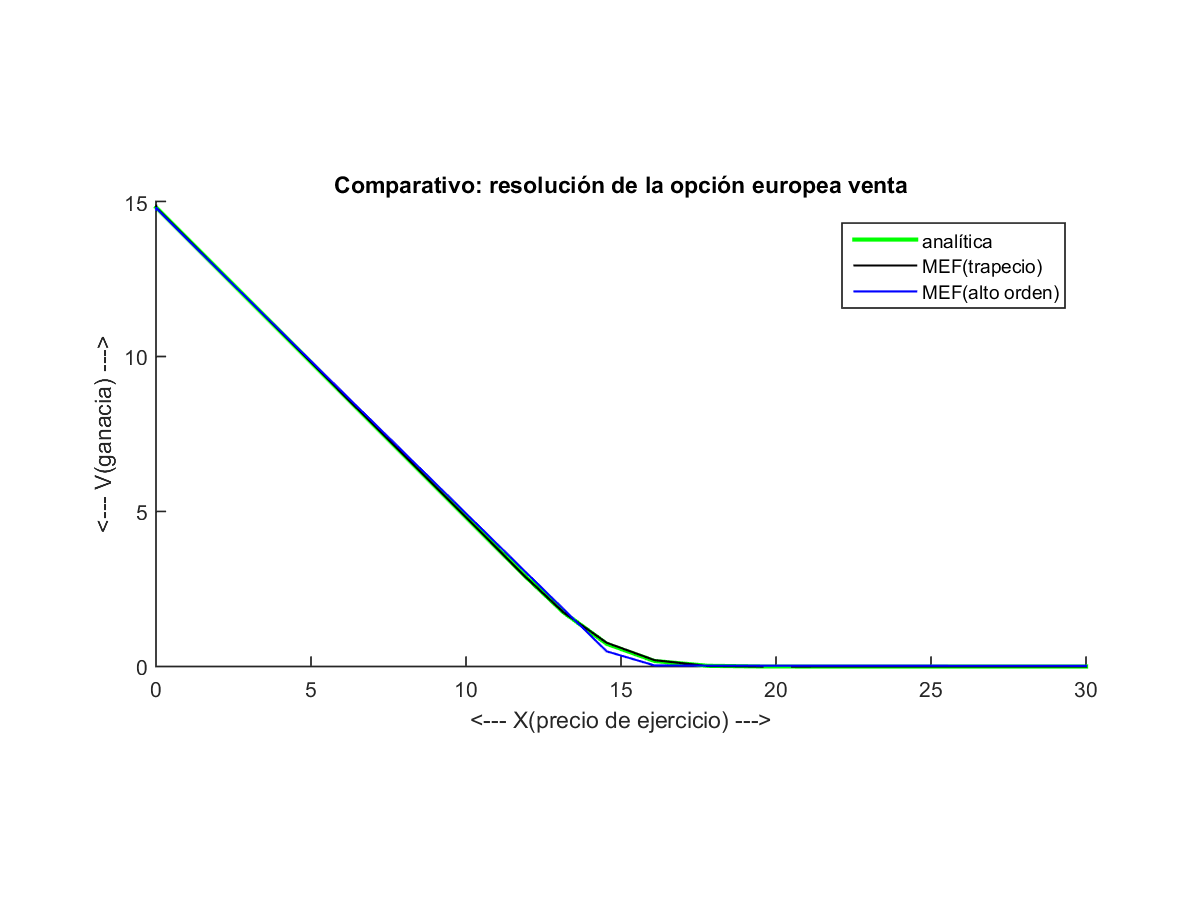
\includegraphics[height=64mm]{Pic/resolucionMEF} &
			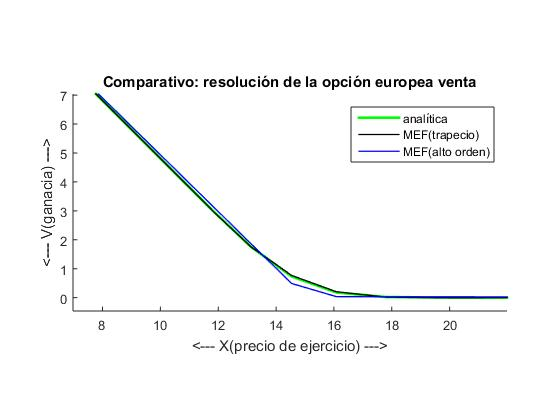
\includegraphics[height=64mm]{Pic/Zoom}
		\end{tabular}
	\hrule
	\end{table}

%%%%%%%%%%%%%%%%%%%%%%%%%%%%%%%%%%%%%%%%%%%%%%%%%%%%%%%%%%%%%%%%555
\subsection{Análisis de convergencia exponecial de error} \label{error}
\begin{figure}[h]
\begin{center}
\begin{tikzpicture}[scale=1]
\begin{loglogaxis}[
xlabel=\textsc{<--- x --->},
ylabel=$L_2$ Error ]
\axispath\draw
(7.49165,-10.02171)
|-  (8.31801,-11.32467)
node[near start,left] {$ $};
\addplot plot coordinates {
	(5,     8.312e-02)
	(17,    2.547e-02)
	(49,    7.407e-03)
	(129,   2.102e-03)
	(321,   5.874e-04)
	(769,   1.623e-04)
	(1793,  4.442e-05)
	(4097,  1.207e-05)
	(9217,  3.261e-06) }; 
\addplot plot coordinates {
	(7,     8.472e-02)
	(31,    3.044e-02)
	(111,   1.022e-02)
	(351,   3.303e-03)
	(1023,  1.039e-03)
	(2815,  3.196e-04)
	(7423,  9.658e-05)
	(18943, 2.873e-05)
	(47103, 8.437e-06) };
\addplot plot coordinates {
	(9, 7.881e-02)
	(49,    3.243e-02)
	(209,   1.232e-02)
	(769,   4.454e-03)
	(2561,  1.551e-03)
	(7937,  5.236e-04)
	(23297, 1.723e-04)
	(65537, 5.545e-05)
	(178177,    1.751e-05) };
\legend{$deg=1$\\$deg=2$\\$deg=3$\\$deg=4$\\$deg=5$\\}
\end{loglogaxis}
\end{tikzpicture}
\end{center}
\hrule
\end{figure}
\vspace{3cm}
\begin{center}
	\textit{La soberanía del hombre está oculta en la dimensión de sus conocimientos}.(Sir F. Bacon)
\end{center}
%%%%%%%%%%%%%%%%%%%%%%%%%%% FIN  %%%%%%%%%%%%%%%%%%%%%%%%%%5
\end{document}